\documentclass[oneside, a4paper, 12pt]{book}

%% подключаем стандарт библиографии
\bibliographystyle{gost71u} 

%% for envirovemt "abstract" in class book
\newenvironment{abstract}{}{}
\usepackage{abstract}
\usepackage{sectsty}
\sectionfont{\centering}
\usepackage{float}
%% подключаем преамбулу, в ней содержатся подключение всех необходимых пакетов
%%% Работа с русским языком
\usepackage{cmap}			 % поиск в PDF
\usepackage{mathtext} 		 % русские буквы в формулах
\usepackage[T2A]{fontenc}	 % кодировка
\usepackage[utf8]{inputenc}	 % кодировка исходного текста
\usepackage[russian]{babel}	 % локализация и переносы

%%% Пакеты для работы с математикой
\usepackage{amsmath,amsfonts,amssymb,amsthm,mathtools}
\usepackage{icomma}

%% Номера формул
%\mathtoolsset{showonlyrefs=true} % Показывать номера только у тех формул, на которые есть \eqref{} в тексте.
%\usepackage{leqno}               % Немуреация формул слева

%% Шрифты
\usepackage{euscript}	 % Шрифт Евклид
\usepackage{mathrsfs}    % Красивый матшрифт

%% Поля (геометрия страницы)
\usepackage[left=3cm,right=2cm,top=2cm,bottom=2cm,bindingoffset=0cm]{geometry}

%% Русские списки
\usepackage{enumitem}
\makeatletter
\AddEnumerateCounter{\asbuk}{\russian@alph}{щ}
\makeatother

%%% Работа с картинками
\usepackage{caption}
\captionsetup{justification=centering} % центрирование подписей к картинкам
\usepackage{graphicx}                  % Для вставки рисунков
\graphicspath{{images/}{images2/}}     % папки с картинками
\setlength\fboxsep{3pt}                % Отступ рамки \fbox{} от рисунка
\setlength\fboxrule{1pt}               % Толщина линий рамки \fbox{}
\usepackage{wrapfig}                   % Обтекание рисунков и таблиц текстом

%%% Работа с таблицами
\usepackage{array,tabularx,tabulary,booktabs} % Дополнительная работа с таблицами
\usepackage{longtable}                        % Длинные таблицы
\usepackage{multirow}                         % Слияние строк в таблице

%% Красная строка
\setlength{\parindent}{2em}

%% Интервалы
\linespread{1}
\usepackage{multirow}

%% TikZ
\usepackage{tikz}
\usetikzlibrary{graphs,graphs.standard}

%% Верхний колонтитул
\usepackage{fancyhdr}
\pagestyle{fancy}
\fancyhead[L]{}


%% Перенос знаков в формулах (по Львовскому)
\newcommand*{\hm}[1]{#1\nobreak\discretionary{}{\hbox{$\mathsurround=0pt #1$}}{}}

%% дополнения
\usepackage{float}   % Добавляет возможность работы с командой [H] которая улучшает расположение на странице
\usepackage{gensymb} % Красивые градусы
\usepackage{caption} % Пакет для подписей к рисункам, в частности, для работы caption*

% подключаем hyperref (для ссылок внутри  pdf)
\usepackage[unicode]{hyperref}
\usepackage{listings}

\begin{document}
    %% титульник
    %%\begin{center}
    %% *название института*
    \large\textbf{Министерство науки и высшего образования Российской Федерации
    Федеральное государственное автономное образовательное учреждение высшего образования
    «Московский физико-технический институт (национальный исследовательский университет)»} \\
    \vspace{1cm}

    %% *факультет/физтех-школа*
    Физтех-школа Радиотехники и Компьютерных Технологий \\

    %% *название базовой кафедры и лаборатории*
    %% в случае ненадобности можно удалить
    Кафедра микропроцессорных технологий в интеллектуальных системах управления \\

    \vspace{3em}

    Выпускная квалификационная работа бакалавра
\end{center}

\begin{center}
    \vspace{\fill}
    %% *название вашей работы*
    \LARGE{Разработка модуля автогенерации платформо-зависимых констант для целей кросс-компиляции}

    \vspace{\fill}
\end{center}


\begin{flushright}
    \textbf{Автор:} \\
    Студент Б01-909а группы \\
    Кофанов Даниил Сергеевич \\
    \vspace{2em}
    \textbf{Научный руководитель:} \\
    *научная степень* \\
    Ишин Павел Андреевич \\
\end{flushright}

\vspace{7em}

\begin{center}
    %% *лого*
    \includegraphics[width=100 pt]{MIPT_logo.jpg}\\
    Москва \the\year{}
\end{center}

% выключаем отображение номера для этой страницы (титульник)
\thispagestyle{empty}

\newpage
\fancyfoot[c]{\thepage}
%% *надпись над верхним колонтинулом*
%% в случае ненадобности можно удалить
\fancyhead[L]{Разработка модуля автогенерации платформо-зависимых констант для целей кросс-компиляции}
\fancyhead[R]{}

    %% аннотоция
    \begin{abstract}

    \begin{center}
        \large{Разработка модуля автогенерации платформо-зависимых констант для целей кросс-компиляции} \\
    \large\textit{Кофанов Даниил Сергеевич} \\[1 cm]
    \end{center}

    \begin{flushleft}
    %% Краткое описание задачи и основных результатов, мотивирующее прочитать весь текст
В Главе 1 данной работе определена практическая ценность кросс-компиляции в контексте виртуальных машин.
В Главе 2 на примере работы абстрактной виртуальной машины дано определение платформо-зависимых констант и сформулирована связанная с ними проблема, возникающая при кросс-компиляции.
В Главе 3 предложена идея гибкого и масштабируемого решения этой проблемы, основанного на создании некоторого интерфейса и использовании системного (т. е. не относящегося к виртуальным машинам) кросс-компилятора.
Произведено сравнение с альтернативным решением.
В Главе 4 дан обзор имплементации найденного решения в виртуальной машине с открытым исходным кодом ArkCompiler, основанного на модуле ExternalProject утилиты cmake.
В Главе 5 отмечены преимущества, включающие высокую степень автоматизированности, удобства в использовании разработанного интерфейса.
Также выделены недостатки текущей имплементации, предложены пути их устранения.
    \end{flushleft}

\end{abstract}

    %содержание
    \tableofcontents{}
    \setcounter{page}{2}
    \newpage

    \chapter{Введение}
\label{sec:Chapter0} \index{Chapter0}

\section{Контекст проблемы}
На момент написания этой работы сложно переоценить влияние мобильных устройств на повседневную жизнь.
Смартфоны предоставляют огромный спектр возможностей, начиная от коммуникации и игр, заканчивая рабочими потребностями, навигацией и отслеживанием физического состояния человека.
Количество использующихся телефонов значительно преобладает над количеством ПК и ноутбуков.
Однако такой массовый характер был бы невозможен в отсутствии многообразия устройств на рынке.
Действительно, развитие технологий безусловно исходит из потребности в новых возможностях, однако финансирование этого развития поступает из уже существующих и отлаженных технологий.
Кроме того, только что изобретённой технологии требуется некоторое время, чтобы спрос на неё появился и вырос.
Исходя из этого, а также готовности потребителя пойти на компромисс между ценой за устройство и количеством и качеством предоставляемых им функций, представленные на рынке устройства коренным образом отличаются между собой.

\par
С другой стороны, имея такое разнообразие, разрабатывать приложения и отлаживать под каждое устройство было бы слишком дорогой задачей.
Чтобы решить эту проблему, вводится понятие виртуальной машины, то есть некоторого абстрактного вычислителя, способного исполнять инструкции из определённого набора, тем самым обеспечивая разработчиков приложений некоторым количеством гарантий.
Кажется очевидным, что этот подход аналогичен договорённости между программистами и разработчиками микропроцессоров в виде архитектуры системы команд и почти в той же степени необходим.
Главное отличие заключается в более высоком уровне абстракции, что позволяет переложить ответственность за управление ресурсами приложения, например выделение и освобождение памяти, на саму виртуальную машину, тем самым упрощая код и снижая требовательность к опыту разработчика.
В случае мобильных устройств, виртуальная машина рассматривается практически как неотъемлемая часть операционной системы, которая, помимо обеспечения гарантий разработчикам приложений, служит барьером безопасности для пользователей, устанавливающих и использующих самые разные приложения. 

\par
Высокоуровневость виртуальных машин позволяет выражать программы более компактно в сравнении с представлением в нативном коде.
В то же время, нативный код, полученный в результате анализа программы целиком, несравнимо быстрее поочерёдного исполнения инструкций виртуальной машины (интерпретации байткода).
Выходом из этой ситуации стало использование Just-In-Time компиляции, то есть генерации оптимизированного нативного кода для часто вызываемых функций, происходящей параллельно выполнению основного алгоритма.
Использование как классических оптимизаций (межпроцедурной оптимизации, раскрутки циклов) так и специфичных JIT-оптимизаций (профилирование типов в случае динамических языков) позволяет достичь производительности, нивелирующей накладные расходы вносимые этим уровнем абстракции.
В виртуальных машинах так же используется Ahead-Of-Time компиляция, производящаяся до запуска приложения.
Это позволяет избежать излишних затрат энергии при повторных запусках приложений связанных с JIT-компиляцией, скомпилировать большее количество методов, и, возможно, применить большее количество оптимизаций, тем самым экономя заряд батареи мобильных устройств, ускоряя время запуска и улучшая производительность приложения ценой хранения результатов компиляции (AOT-файлов) на устройстве.

\par
Очевиден тот факт, что множество приложений в своих подзадачах часто используют идентичные алгоритмы, такие как сортировка, работа со строками и т. д., и что множественная имплементация того или иного алгоритма ведёт к практической сложности поддержки такого кода.
Ввиду этого, многие алгоритмы, оптимизированные с целью быть приемлимо эффективными для самых различных нагрузок, образуют стандартную библиотеку языка и поставляются вместе с виртуальной машиной.
Будучи часто переиспользуемой, стандартная библиотека AOT-компилируется и хранится на устройстве, что позволяет любому приложению гарантировано использовать оптимизированный нативный код, не совершая излишнюю работу по JIT-компиляции.

\par
Выпуская огромное количество устройств, запуск AOT-компиляции стандартной библиотеки на каждом из них был бы нерационален и сопровождался бы ощутимыми издержками производства.
Их можно избежать путём единовременной компиляции и последующей загрузки полученного образа на устройства, например при прошивке.
Для подготовки образа виртуальной машины и операционной системы используется специальный набор утилит, включающий в себя кросс-компилятор и опции компиляции, который работает на отличной от целевого устройства платформе и генерирующий исполняемые файлы в виде нативного кода целевого устройства.
Для такого набора утилит принят термин таргет-тулчейн, в то время как для аналогичного набора утилит, предназначенных для получения исполняемых файлов для той же платформы на которой они и были сгенерированы, используется термин хост-тулчейн.

\par
Однако, таргет-тулчейн не подходит для непосредственной подготовки AOT-файла стандартной библиотеки.
Это связано с тем, что стандартная библиотека рассчитана на исполнение в среде виртуальной машины, отличающейся от окружения создаваемого операционной системой и может проявляться в том, что тулчейн-компилятор и AOT-компилятор виртуальной машины могут использовать разное соглашение о вызовах.
Поэтому приобретает смысл вопрос о кросс-компиляторе в терминах виртуальной машины, что на самом деле означает возможность генерации AOT-файлов виртуальной машины для определённого устройства на другой платформе, например на сервере. Эта задача имеет множество тонкостей, одной из которых посвящена данная работа - проблема зависимости некоторых численных значений от платформы (платформо-зависимых констант).
Наиболее ярким примером является размер указателя.
Однако в этом случае зависимость от платформы достаточно легко <<предсказать>>: на AMD64-совместимой платформе это скорее всего 8 байт, а на ARM32 - 4.
Другим, более трудноразрешимым и содержательным примером является смещение до полей в структурах данных.
Даже в процессе компиляции на одной и той же платформе одним и тем же компилятором, в зависимости от опций компиляции результат может быть различным.
В последующих главах излагается подробное описание этой проблемы, на примере абстрактной виртуальной машины демонстрируется один из источников таких значений, а также предлагается решение, основанное на использовании таргет-тулчейна, нашедшее применение в некоторой виртуальной машине.
Как будет показано в дальнейшем, эта имплементация отличается высоким уровнем автоматизации и масштабируемости, делающей её малозаметной и лёгкой в использовании.
Кроме того, помимо основной функции, она вносит дополнительную степень верификации AOT-файлов.

\section[Описание проблемы]{Описание проблемы на практическом примере}
Рассмотрим более подробно язык программирования, который поддерживает какая-либо представляющая интерес виртуальная машина, реализованная, для определённости, на языке C++.
Положим также, что в нём существуют некоторые встроенные типы, это могут быть числа, строки массивы, словари и т.д., а операции с этими сущностями, например их создание, модификация, получение внутреннего состояния, выражаются в специальных инструкциях виртуальной машины.
Тогда при исполнении программы созданию массива будет соответствовать выполнение некой инструкции \textit{newarray}, а получению длины этого массива -- выполнение \textit{arraylength} (рис. 2.1).

\begin{figure}[H]
    \centering
    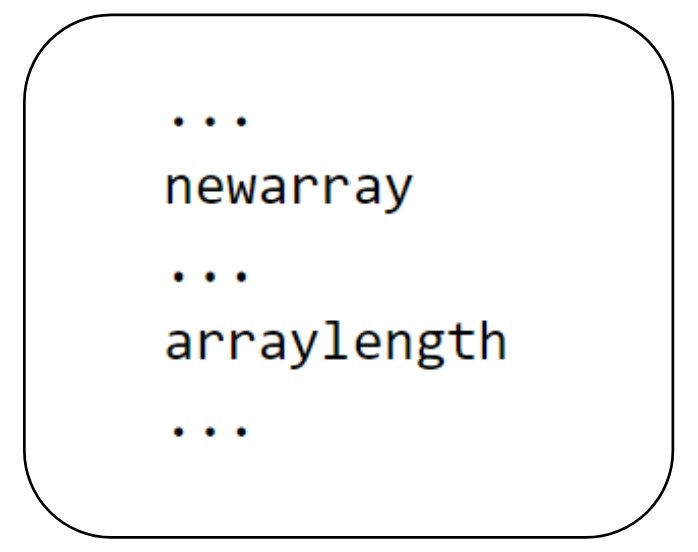
\includegraphics[scale=0.7]{bytecodes_array.jpg}
    \caption{Пример инструкций в программе}
\end{figure}

С другой стороны, каждый встроенный тип находит отражение в некотором C++-классе. При этом, при исполнении инструкции \textit{newarray} будет происходить аллокация экземпляра этого класса, а при исполнении \textit{arraylength} будет произведено чтение поля \textit{size\_} одного из экземпляров (рис. 2.2).

\begin{figure}[H]
    \centering
    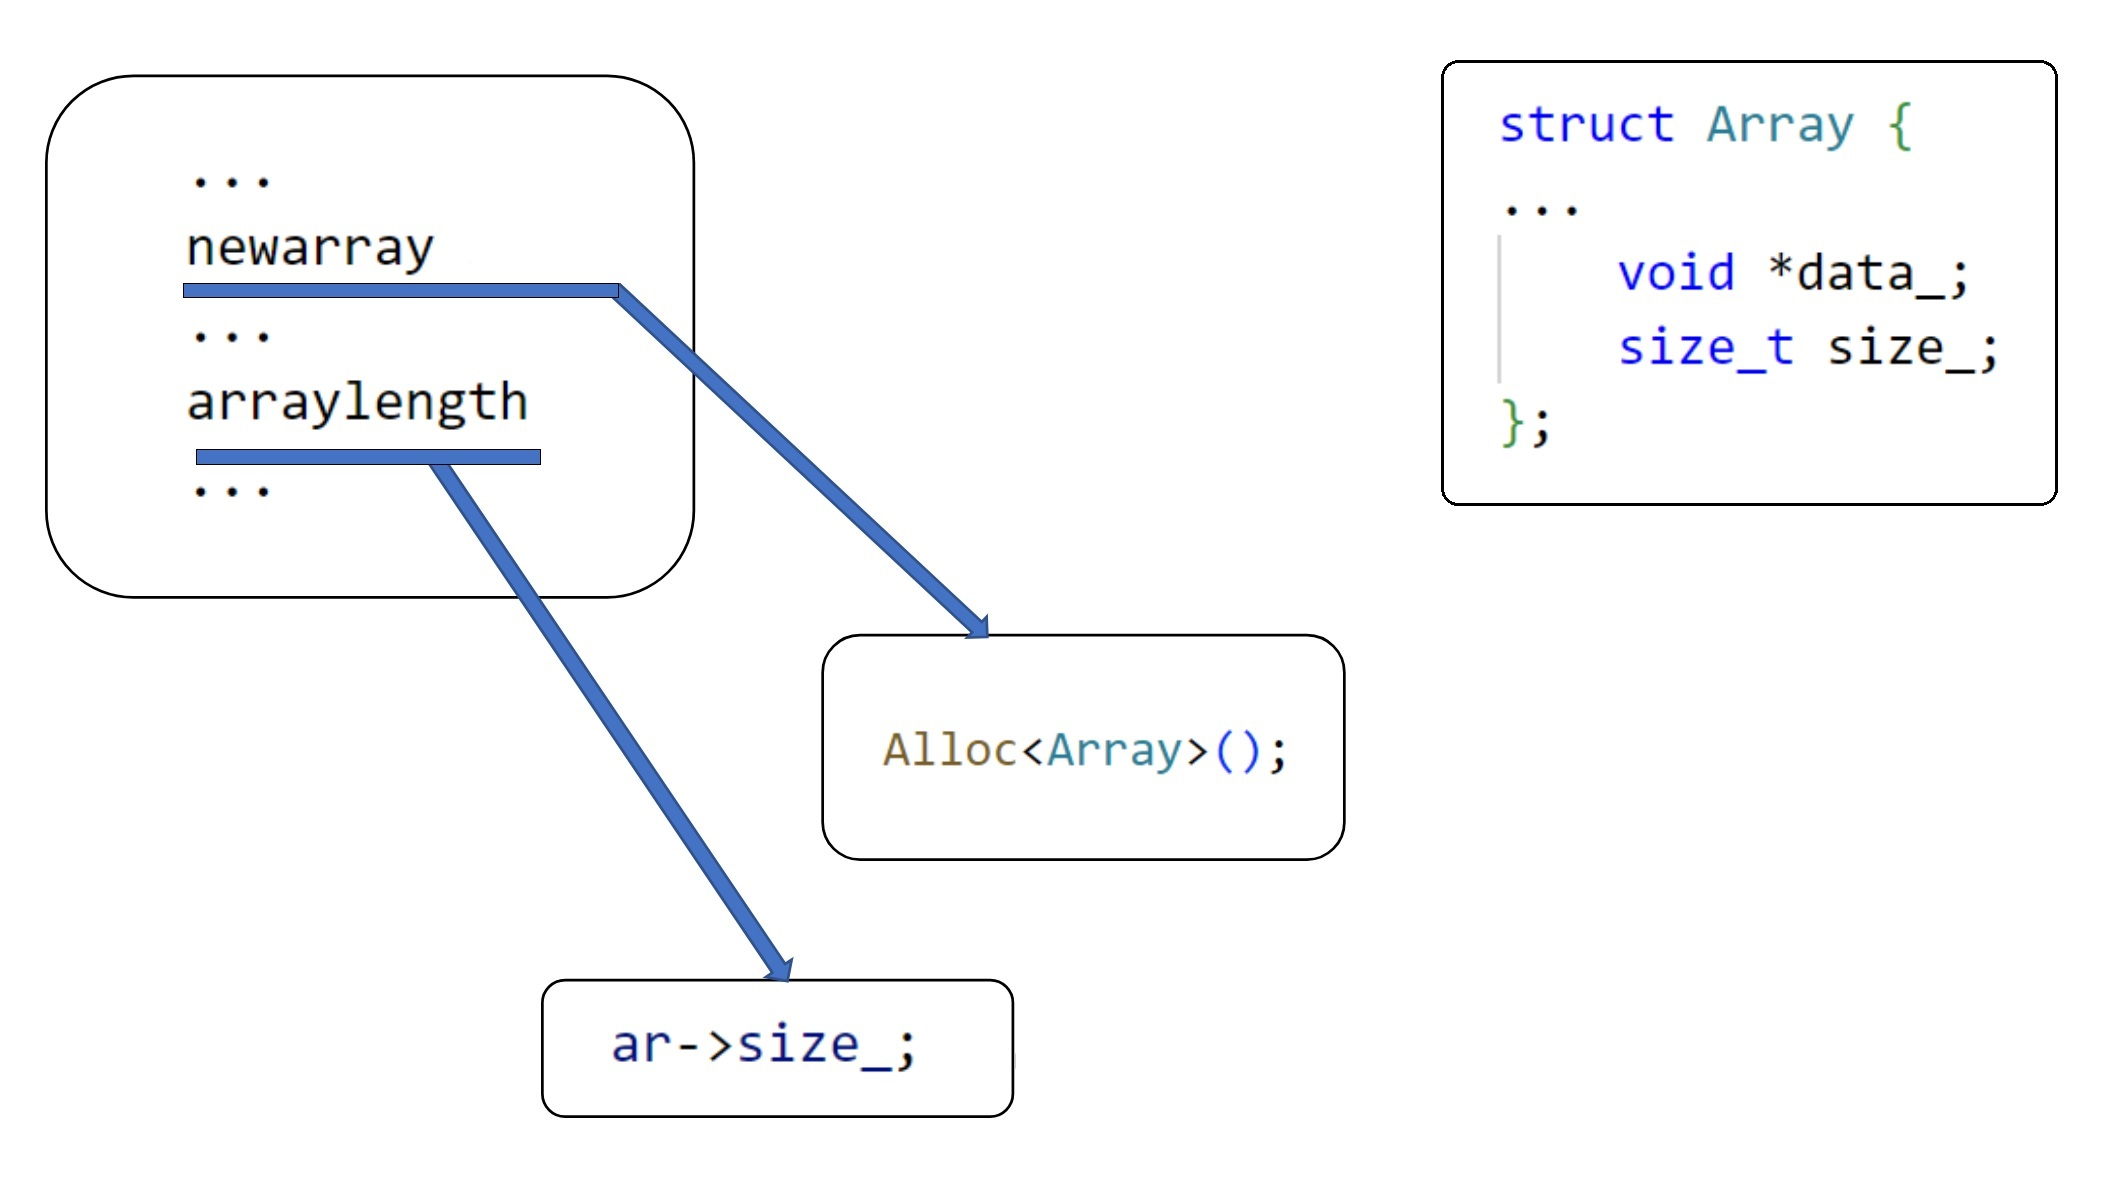
\includegraphics[scale=0.5]{mirror_class.jpg}
    \caption{Реализация семантики языка}
\end{figure}

В нативном формате обращение к этому полю будет выражено в виде машинной инструкции загрузки по указателю с константным смещением.
Возвращаясь к кросс-компилятору виртуальной машины, эта инструкция будет создана на финальном этапе, кодогенерации, из соответствующей инструкции промежуточного представления.
Фактически, эта инструкция промежуточного представления абстрагирует бинарный формат машинной инструкции загрузки по смещению конкретной архитектуры, отделяя зависимость от платформы.
Однако, такой абстракции для отделения оказывается недостаточно.
\par
Дело в том, что смещение до поля класса (эквивалентное в рассматриваемой ситуации смещению в инструкции загрузки), в общем случае, зависит от платформы.
Это может происходить по разным причинам, например -- из-за зависимости размера какого-либо элемента структуры данных от платформы, выравнивания по разным адресам.
Так, рассматриваемое ранее смещение до поля \textit{size\_} структуры \textit{Array} на 64-битной архитектуре AMD64 будет равно 8 байтам, хотя на архитектуре ARM32 -- 4.
Если упустить из рассмотрения этот факт, то кросс-компилятор виртуальной машины, запущенный на AMD64-сервере, при генерации ARM32-инструкций будет использовать соответствующее текущей платформе значение смещения.
Тогда, при запуске такого кода на ARM32-телефоне, исполнение такой инструкции приведёт к некорректному поведению и будет являться программной уязвимостью.
Вопрос корректности и безопасности генерируемого кода является первостепенным в процессе компиляции, что подчёркивает значимость этой проблемы.
\par
Можно выделить два подхода, позволяющие разрешить этот конфликт: первый -- сделать смещения для всех платформ одинаковыми, второй -- каким-либо образом сообщать компилятору значение константы на платформе, для которой происходит компиляция. Данная работа посвящена главным образом реализации второго из них, однако в следующих главах также производится сравнение этих подходов, обосновывающее этот выбор.

\section{Терминология}
Для дальнейшего повествования удобно ввести следующие определения.

\begin{itemize}
    \item
        \textit{Тулчейн} -- набор утилит, позволяющий транслировать C++-программы в некоторый бинарный код.
    \item
        \textit{Платформа} -- предполагаемое тулчейном окружение, в котором будет исполняться сгенерированный им код. Подразумевается, что каждая платформа в достаточной степени однозначно определяется некоторым тулчейном. В качестве синонима, в данной работе может также использоваться термин \textit{архитектура}.
    \item
        \textit{Хост-тулчейн} -- тулчейн предназначенный для генерации кода, совместимого с той же платформой, на которой и генерируется.
    \item
        \textit{Таргет-тулчейн} -- тулчейн предназначенный для генерации кода, совместимого с платформой отличной от той, на которой был сгенерирован.
    \item
        \textit{Платформо-зависимая константа} -- именованное, определённое в терминах C++ константное выражение, численное значение которой каким-либо образом зависит от платформы. Под этим термином может пониматься как множество численных значений какой-либо величины на всех платформах, так и само значение на какой-то конкретной платформе.
    \item
        \textit{Гостевая константа} -- значение платформо-зависимой константы, соответствующее некоему таргет-тулчейну.
\end{itemize}

\newpage %% Введение
    \chapter{Постановка задачи}
\label{sec:Chapter1} \index{Chapter1}

Примем следующие определения.

\begin{itemize}
    \item
        \textit{Тулчейн} - набор утилит, позволяющий транслировать C++-программы в некоторый бинарный код.
    \item
        \textit{Платформа} - предполагаемое тулчейном окружение, в котором будет исполняться сгенерированный им код. Подразумевается, что каждая платформа в достаточной степени однозначно определяется некоторым тулчейном. В качестве синонима, в данной работе будет также использоваться термин \textit{архитектура}.
    \item
        \textit{Платформо-зависимая константа} - имеющее определённое имя, определённое в терминах C++ константное выражение, численное значение которой каким-либо образом зависит от платформы.
\end{itemize}

Целью данной работы является разработка модуля, способного каким-либо способом вычислять заранее обговорённый набор платформо-зависимых констант для интересующих разработчика платформ, а так же имеющего интерфейс, предоставляющий доступ к значению любой из констант на каждой из архитектур.
\newpage %% Постановка задачи
    \chapter{Сравнение подходов к проблеме платформо-зависимых констант}
\label{sec:Chapter2} \index{Chapter2}

В этой главе описываются два подхода к решению проблемы платформо-зависимых величин -- фиксирование величин между всеми платформами и, контрастное ему, вычисление величин для каждой платформы, а также производится сравнение этих подходов. Хочется отметить, что данная работа посвящена последнему из них, а так же что её возникновение обязано успешной попытке устранить недостатки, связанные с первым подходом.

\section{Фиксирование констант}
Этот подход заключается в поддержании кода в таком состоянии, при котором величины будут иметь одно и то же значение на каждой из платформ.
Из достоинств данного подхода можно отметить простоту идеи, однако на практике, следование такому подходу сопровождается нетривиальными сложностями.
\par
Например, к этому может привести использование атрибутов, не относящихся к стандарту языка.
При использовании разных тулчейнов, хотя и относящихся к одной и той же платформе (например GCC и LLVM), может получаться отличающийся результат.
\par
Далее, остаётся открытым вопрос самого фиксирования этих величин: ранее был рассмотрен лишь один из примеров -- смещения полей в структуре данных, однако фиксирование величин другой природы может быть связано со значительными сложностями, если будет возможно в принципе.
\par
Кроме этого, для верификации, каждой константе должна соответствовать статическая проверка на то, что текущее значение велчичины действительно совпадает с некоторым жёстко закодированным числом.
Из-за этого, исходный код проекта приобретает избыточную и малоинформативную логику, необходимую лишь для проверки корректности самого подхода, причём на фоне большого числа таких констант сложно гарантировать существование такой проверки для каждой из них.
Более того, при активной разработке и модификации виртуальной машины, фактические значения констант могут меняться (что можно легко проследить на примере изменения смещений при добавлении нового поля в структуру), инициируя необходимость модификации уже существующих проверок.
Разработчик неизбежно будет сталкиваться с последствиями такого подхода, поддержка проекта будет становиться всё сложнее.

\section{Вычисление констант}

Альтернативой является более консервативный подход, описываемый как вычисление величин для каждой платформы и имплементированный в ходе данной работы.
Под консервативностью следует понимать отсутствие каких-либо требований и ограничений, описанных ранее, на значения констант и отсутствие вмешательств в исходный код, связанных с этими ограничениями. Хотя на первый взгляд способ вычисления <<гостевых>> значений кажется неочевидным, предположив что он существует, множество описанных ранее проблем устраняются сами собой или вовсе лишены смысла.

\par
Так, не появляются затруднения при использовании платформо-зависимого функционала какого-либо тулчейна.
Также, не приходится изобретать способ фиксирования для констант разного происхождения, что делает такой подход более однородным и гибким.
Не возникает и вопроса сверки констант на разных платформах, так как разрешается их различие.
Это в свою очередь допускает решения, являющимися локально оптимальными для каждой из платформ.
Например, рассмотрим структуру данных состоящую из двух 32-битных полей. Выравнивание на 8 байт на некой 32-битной архитектуре будет связано с накладными расходами на количество используемой памяти, в то время как выравнивание на 4 байта может повлечь снижение производительности на 64-битной платформе.
Данный подход позволяет использовать 4-байтное выравнивание на 32-битной платформе и 8-байтное выравнивание на 64-битной платформе для одной и той же структуры данных.

\par
Таким образом, этот подход, а именно отказ от <<модификации>> констант, устраняет большинство, если не все, недостатки, описанные в предыдущей секции.
С другой стороны, формально он допускает раннее описанный подход, то есть в определённом смысле не противоречит ему: значения каждой из величин на всех платформах могут (искусственным или естественным образом) совпасть.
С практической точки зрения это означает, что миграция с использования первого подхода на использование второго может происходить поэтапно, то есть сначала можно наладить инфраструктурную часть, а затем, по мере необходимости, ослаблять введённые искусственно ограничения.

\par
Важно сделать следующее замечание.
Необходимо, чтобы полученный кросс-компилятором, расчитывающим на какую-то конкретную платформу, код действительно запускался в контексте виртуальной машины, собранной для той же платформы.
В описываемой ниже имплементации эта проблема устраняется путём вычисления контрольной суммы CRC32 из значений констант на таргет-платформе и последующей её записи как в каждый AOT-файл, генерируемый кросс-компилятором виртуальной машины, так и в сам таргет-образ виртуальной машины.
Во время инсталяции AOT-файла происходит сверка этих значений, что позволяет обнаружить потенциальные ошибки, связанные с несовместимостью между кросс-скомпилированным кодом и самой виртуальной машиной.
Однако в таком виде, эта особенность не является недостатком.
Действительно, значение какой-либо константы может изменяться в зависимости от версии виртуальной машины, а совпадение версии кросс-компилятора, находящегося на сервере, и самой виртуальной машины, находящейся на устройстве, при ошибках инфраструктуры может нарушиться.
Такая контрольная сумма вносит дополнительную степень верификации, косвенно проверяя совместимость версий и несёт дополнительную полезную нагрузку, никак не связанную с выбранным подходом. 

\section{Итог сравнения}
Исходя из вышесказанного, второй подход, связанный с вычислением констант для каждой платформы, является более предпочтительным в виду своей универсальности.
Характерная ему однородность, определённая выше, позволяет в высокой степени автоматизировать весь процесс, связанный с вычислением значений и поддержанием их в консистентном состоянии (как в случае чистой, так и инкрементальной сборки), фактически отделяясь в независимый инкапсулирующий модуль.
Разработчик сталкивается с этим модулем лишь через интерфейс и у него нет необходимости вручную вносить изменения в этот модуль: достаточно лишь определения платформо-зависимой константы, после чего её можно использовать в основной части проекта.

\par
Дальнейшее повествование раскрывает детали реализации выбранного подхода.
 
\newpage %% Обзор существующих решений
    \chapter[Реализация модуля]{Реализация модуля автогенерации платформо-зависимых констант}
\label{sec:Chapter3} \index{Chapter3}

\section{Описание основной идеи решения}
В дальнейшем для определённости предполагается, что исходный код виртуальной машины собирается с помощью утилиты CMake \cite{cmake}.
Данная утилита поддерживает кросс-сборки, позволяя выбрать не только архитектуру микропроцессора, но также уточнить операционную систему целевого устройства (или её отсутствие).
Это позволяет генерировать образы программ под большое множество устройств.
В случае виртуальной машины, подготовив на сервере соответствующий образ и загрузив его на телефон, получается корректно работающая виртуальная машина, способная исполнять байткод, каким-либо образом попадающий на устройство в дальнейшем, а также имеющая JIT- и AOT-компилятор (рис. \ref{fig:device_image}).

\begin{figure}[H]
    \centering
    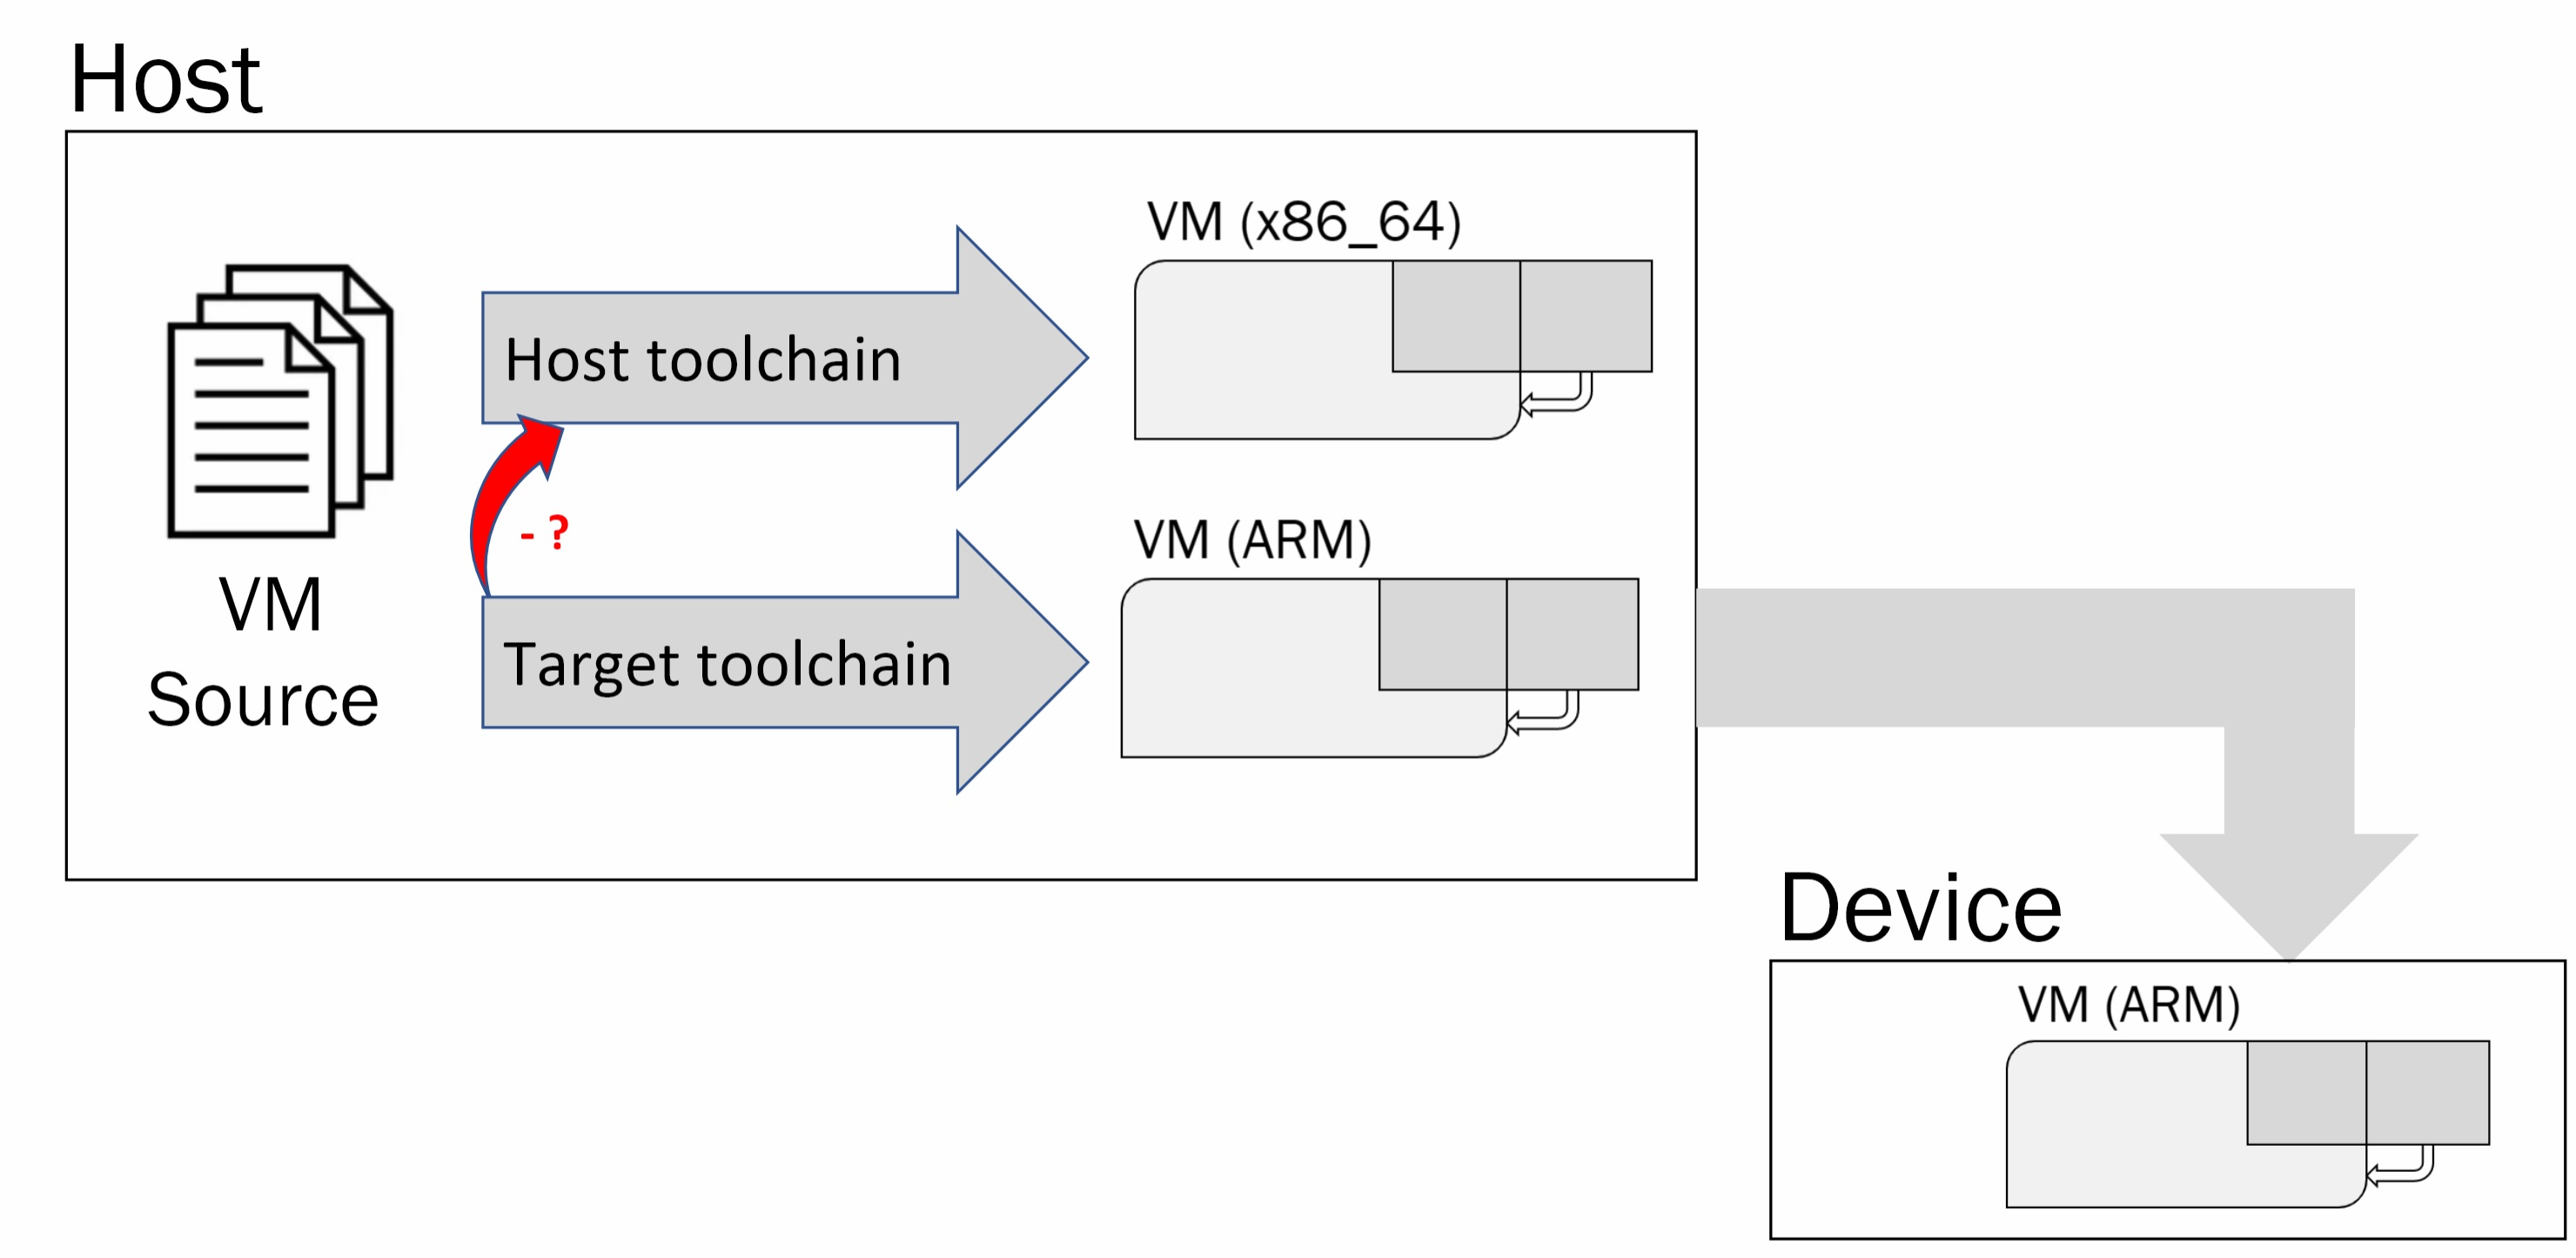
\includegraphics[scale=0.3]{device_image.jpg}
    \caption{Процесс появления виртуальной машины на таргет-устройстве. Под красной стрелкой можно понимать проблему вычисления гостевых констант.}
    \label{fig:device_image}
\end{figure}

Чтобы иметь возможность подготавливать AOT-файлы для телефона на сервере (мотивация чего описана в Главе \ref{sec:Chapter0}), можно каким-либо образом извлечь значения гостевых констант из процесса сборки образа для гостевого устройства и добавить их в некотором виде в исходный код хост-сборки AOT-компилятора.
Идея компактной <<псевдо-сборки>>, которая не полностью подготавливает образ виртуальной машины, а служит лишь для извлечения необходимой информации, и является основной идеей описываемого решения.

\section{Схема вычисления гостевых констант}
Для начала, все платформо-зависимые константы объединяются в специальную единицу трансляции, формат которой приведён на рис. \ref{fig:asm_defines}.

\begin{figure}[H]
    \centering
    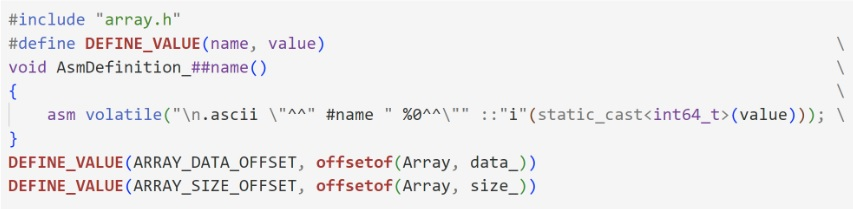
\includegraphics[scale=1.5]{asm_defines.jpg}
    \caption{Формат описываемой единицы трансляции с примером платформо-зависимых констант (смещения до полей структуры \textit{Array}).}
    \label{fig:asm_defines}
\end{figure}

\definecolor{myred}{rgb}{0.5,0,0}
\definecolor{mygr}{rgb}{0,0.5,0}
\definecolor{mygray}{rgb}{0.2,0.2,0.2}
Помимо своего основного предназначения, речь о котором пойдёт далее, она обладает важным документирующим свойством: все платформо-зависимые константы оказываются определены в общем, предназначенном для них месте, а для добавления новой константы требуется лишь добавить строчку формата \lstinline[language=c++, keywordstyle=\color{myred}, keywordstyle=\bfseries\color{myred}, basicstyle=\color{blue}, commentstyle = \ttfamily\color{mygr}, morekeywords={*, DEFINE_VALUE}, breaklines=true, backgroundcolor=\color{gray}]{DEFINE_VALUE(/* id */, /* constant expression */)}.
\par
Далее, рассмотрим подробнее процесс сборки виртуальной машины из исходного кода для хост-устройства.
На стадии CMake-конфигурации помимо основной, хост-сборки, также конфигурируется с использованием соответствующего таргет-тулчейна один или несколько вспомогательных сборок, каждая из которых находится в отдельной директории внутри корневой директории сборки (рис. \ref{fig:build_dir}).

\begin{figure}[H]
    \centering
    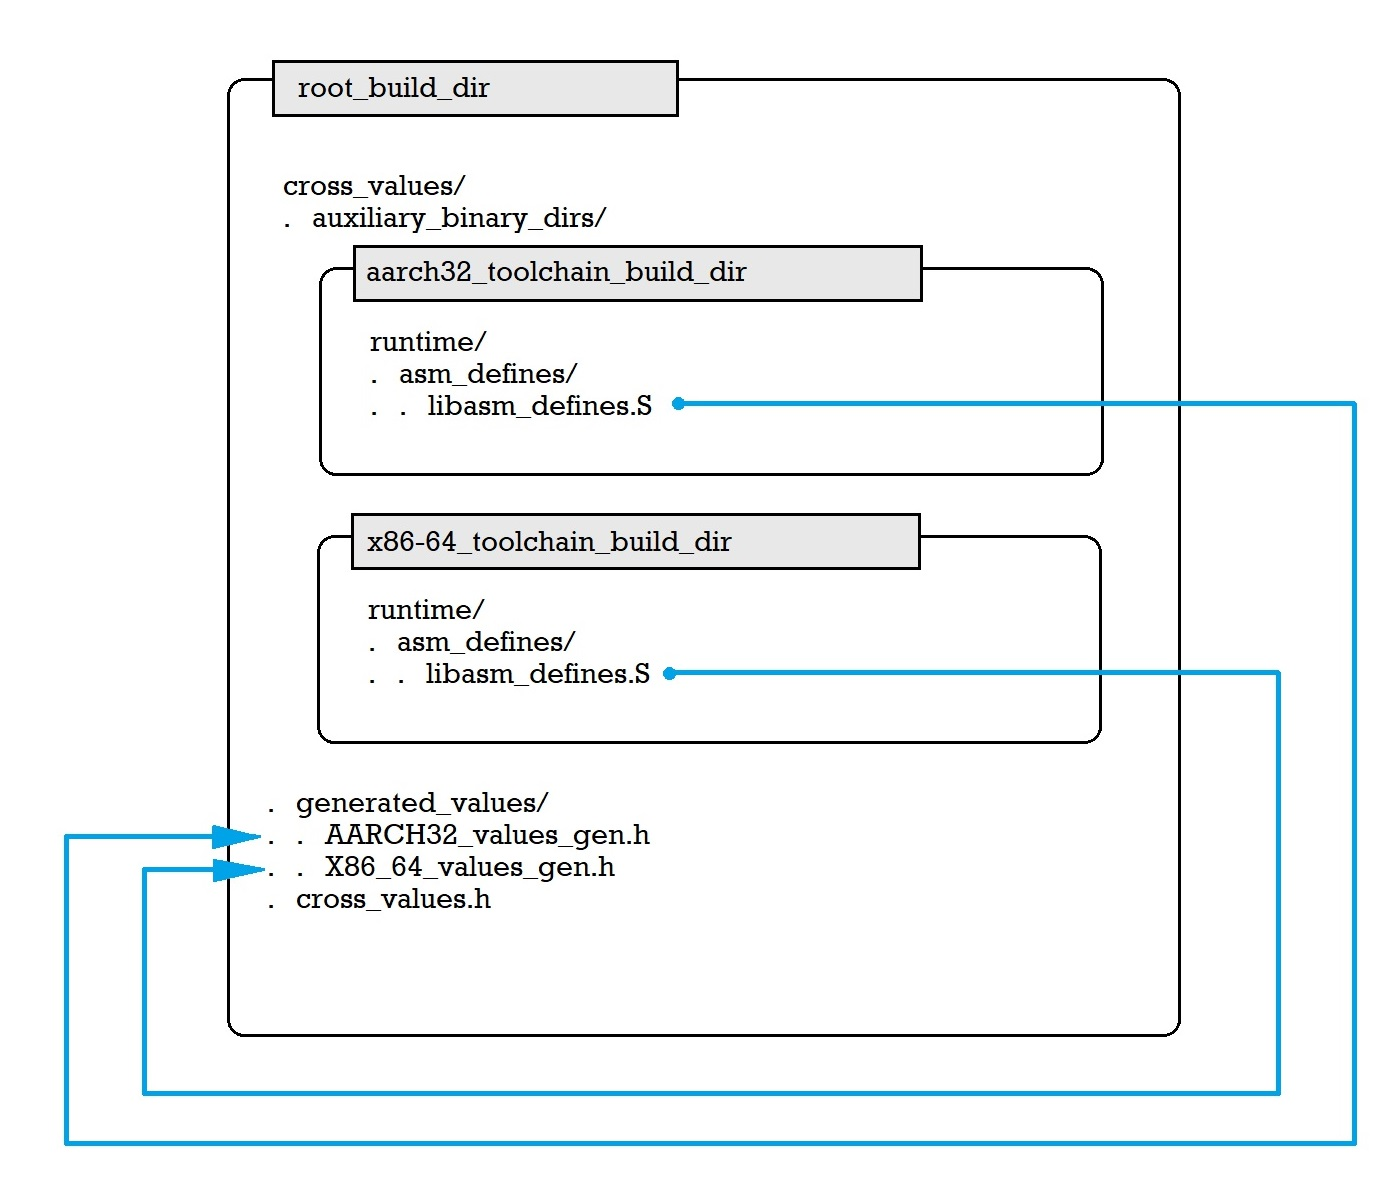
\includegraphics[scale=0.8]{build_dir.jpg}
    \caption{Схема директории сборки виртуальной машины. Голубым цветом обозначены зависимости сборки.}
    \label{fig:build_dir}
\end{figure}

Стоит отметить, что хост-платформа также может рассматриваться как одна из таргет-платформ, что показано на схеме выше.
Это позволяет унифицировать подход к выбору целевой платформы в случае поддержки AOT-компилятором виртуальной машины нескольких целевых платформ.
В каждой вспомогательной сборке, после того как она была сконфигурирована, происходит кросс-компиляция описанной выше единицы трансляции, однако не в бинарный, а ассемблерный вид. Часть такого файла изображена на рисунке \ref{fig:asm_defines_comp}.

\begin{figure}[H]
    \centering
    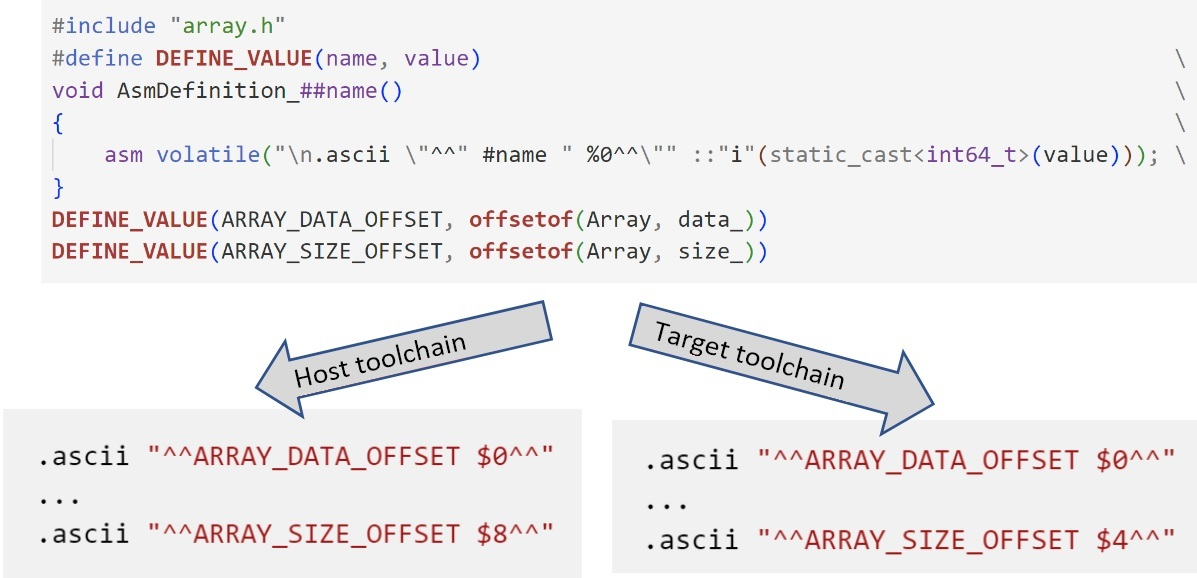
\includegraphics[scale=1]{asm_defines_comp.jpg}
    \caption{Процесс генерации ассемблерного файла с помощью таргет-тулчейнов.}
    \label{fig:asm_defines_comp}
\end{figure}

Особый формат ассемблерных вставок, в которые преобразуются макросы, соответствующие платформо-зависимым константам, позволяют достаточно просто проанализировать результат компиляции и извлечь гостевые константы в численном виде.
Полученные таким образом данные используются для определения C++-констант, имеющих одинаковые имена и разделённые пространством имён, соответствующие обозначению целевой платформы. Они оформляются в виде заголовочных файлов, которые уже могут встраиваться в платформо-специфичный код виртуальной машины, предоставляя тем самым доступ к платформо-зависимым константам (рис. \ref{fig:asm_defines_gen}).

\begin{figure}[H]
    \centering
    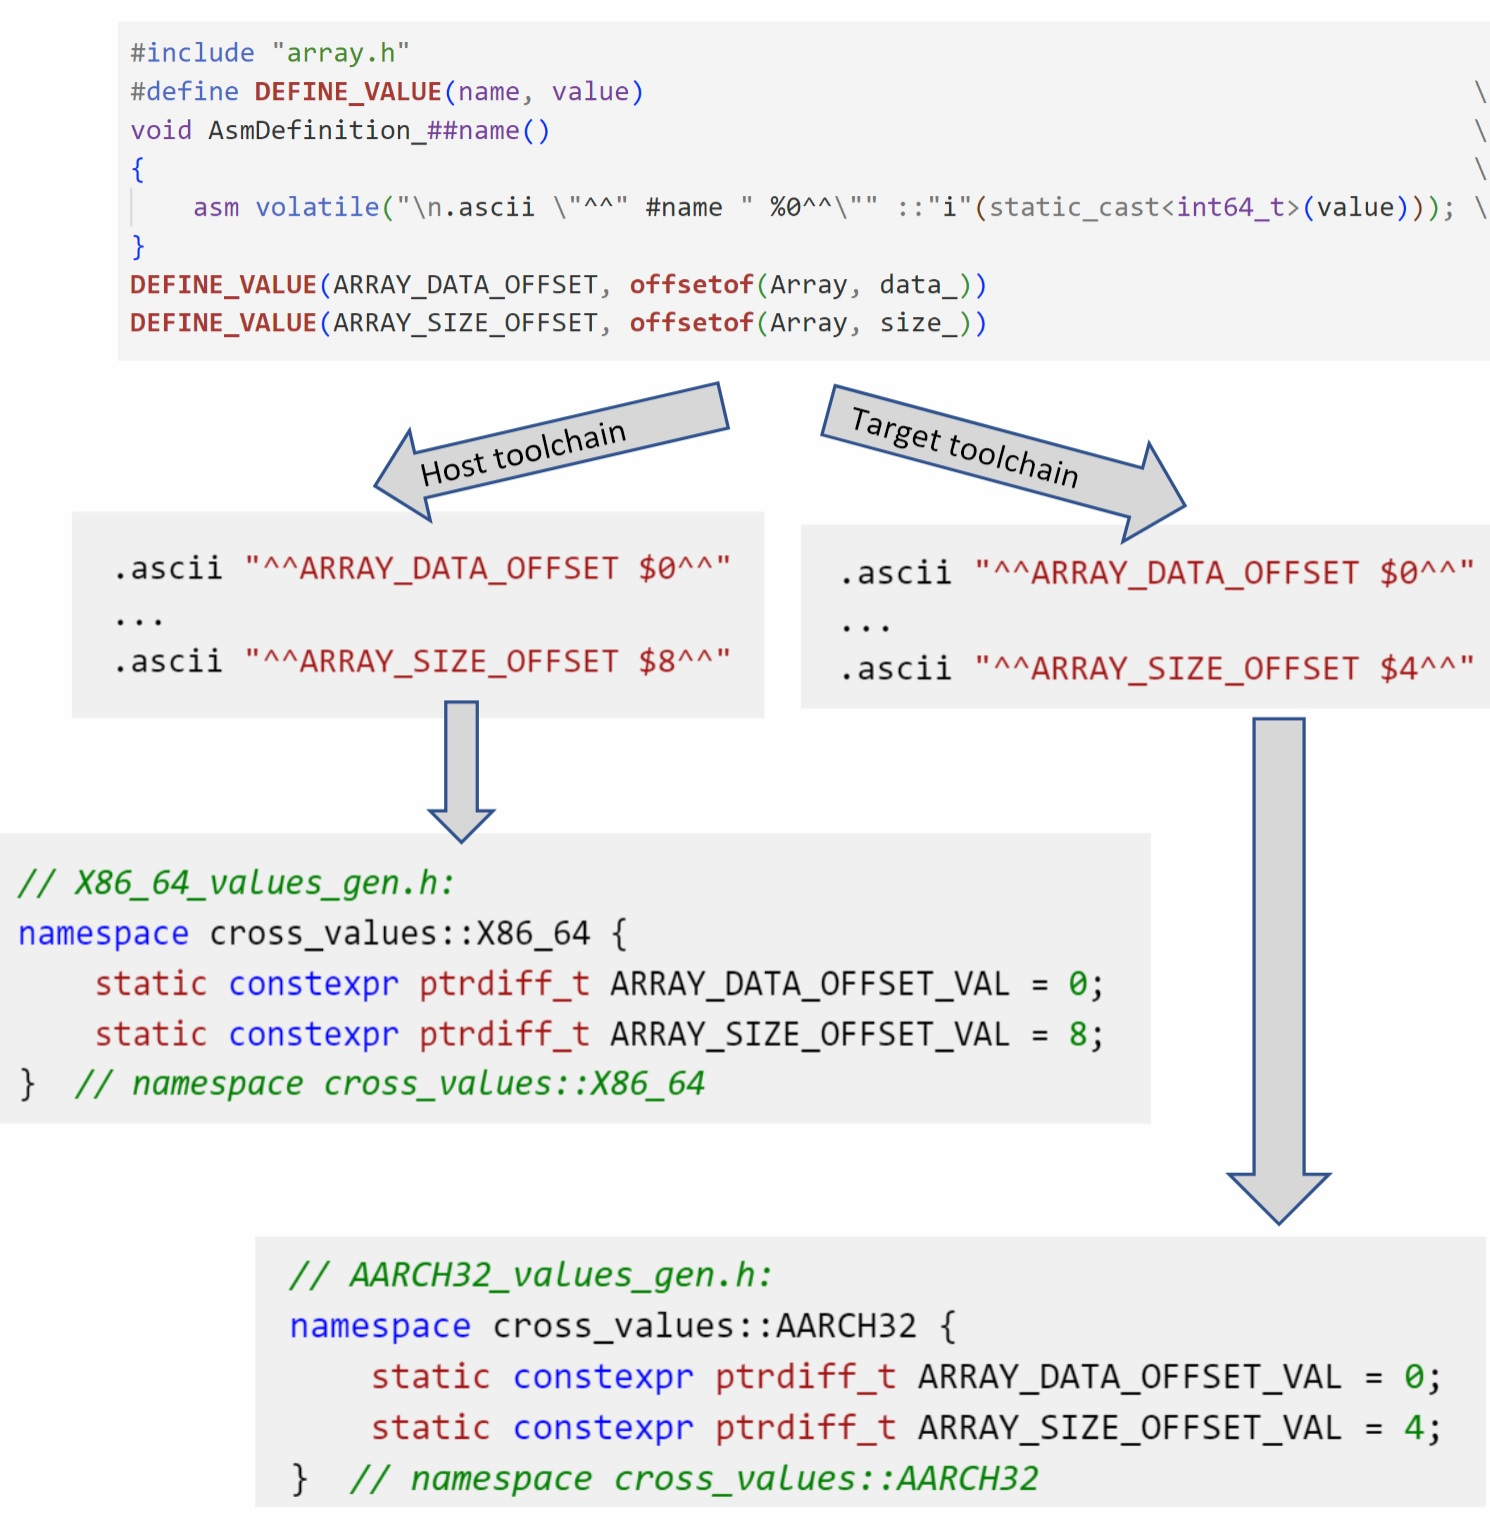
\includegraphics[scale=0.8]{asm_defines_gen.jpg}
    \caption{Схема генерации файлов, содержащих определения констант.}
    \label{fig:asm_defines_gen}
\end{figure}

После того как последний заголовочный файл сгенерирован, необходимо объединить их в один для удобства, а также сгенерировать для каждой платформо-зависимой константы геттер-функцию, позволяющую различать значения каждой из констант, принимаемые ими на целевых платформах, по некоторой переменной перечисляемого типа (рис. \ref{fig:asm_defines_getters}).

\begin{figure}[H]
    \centering
    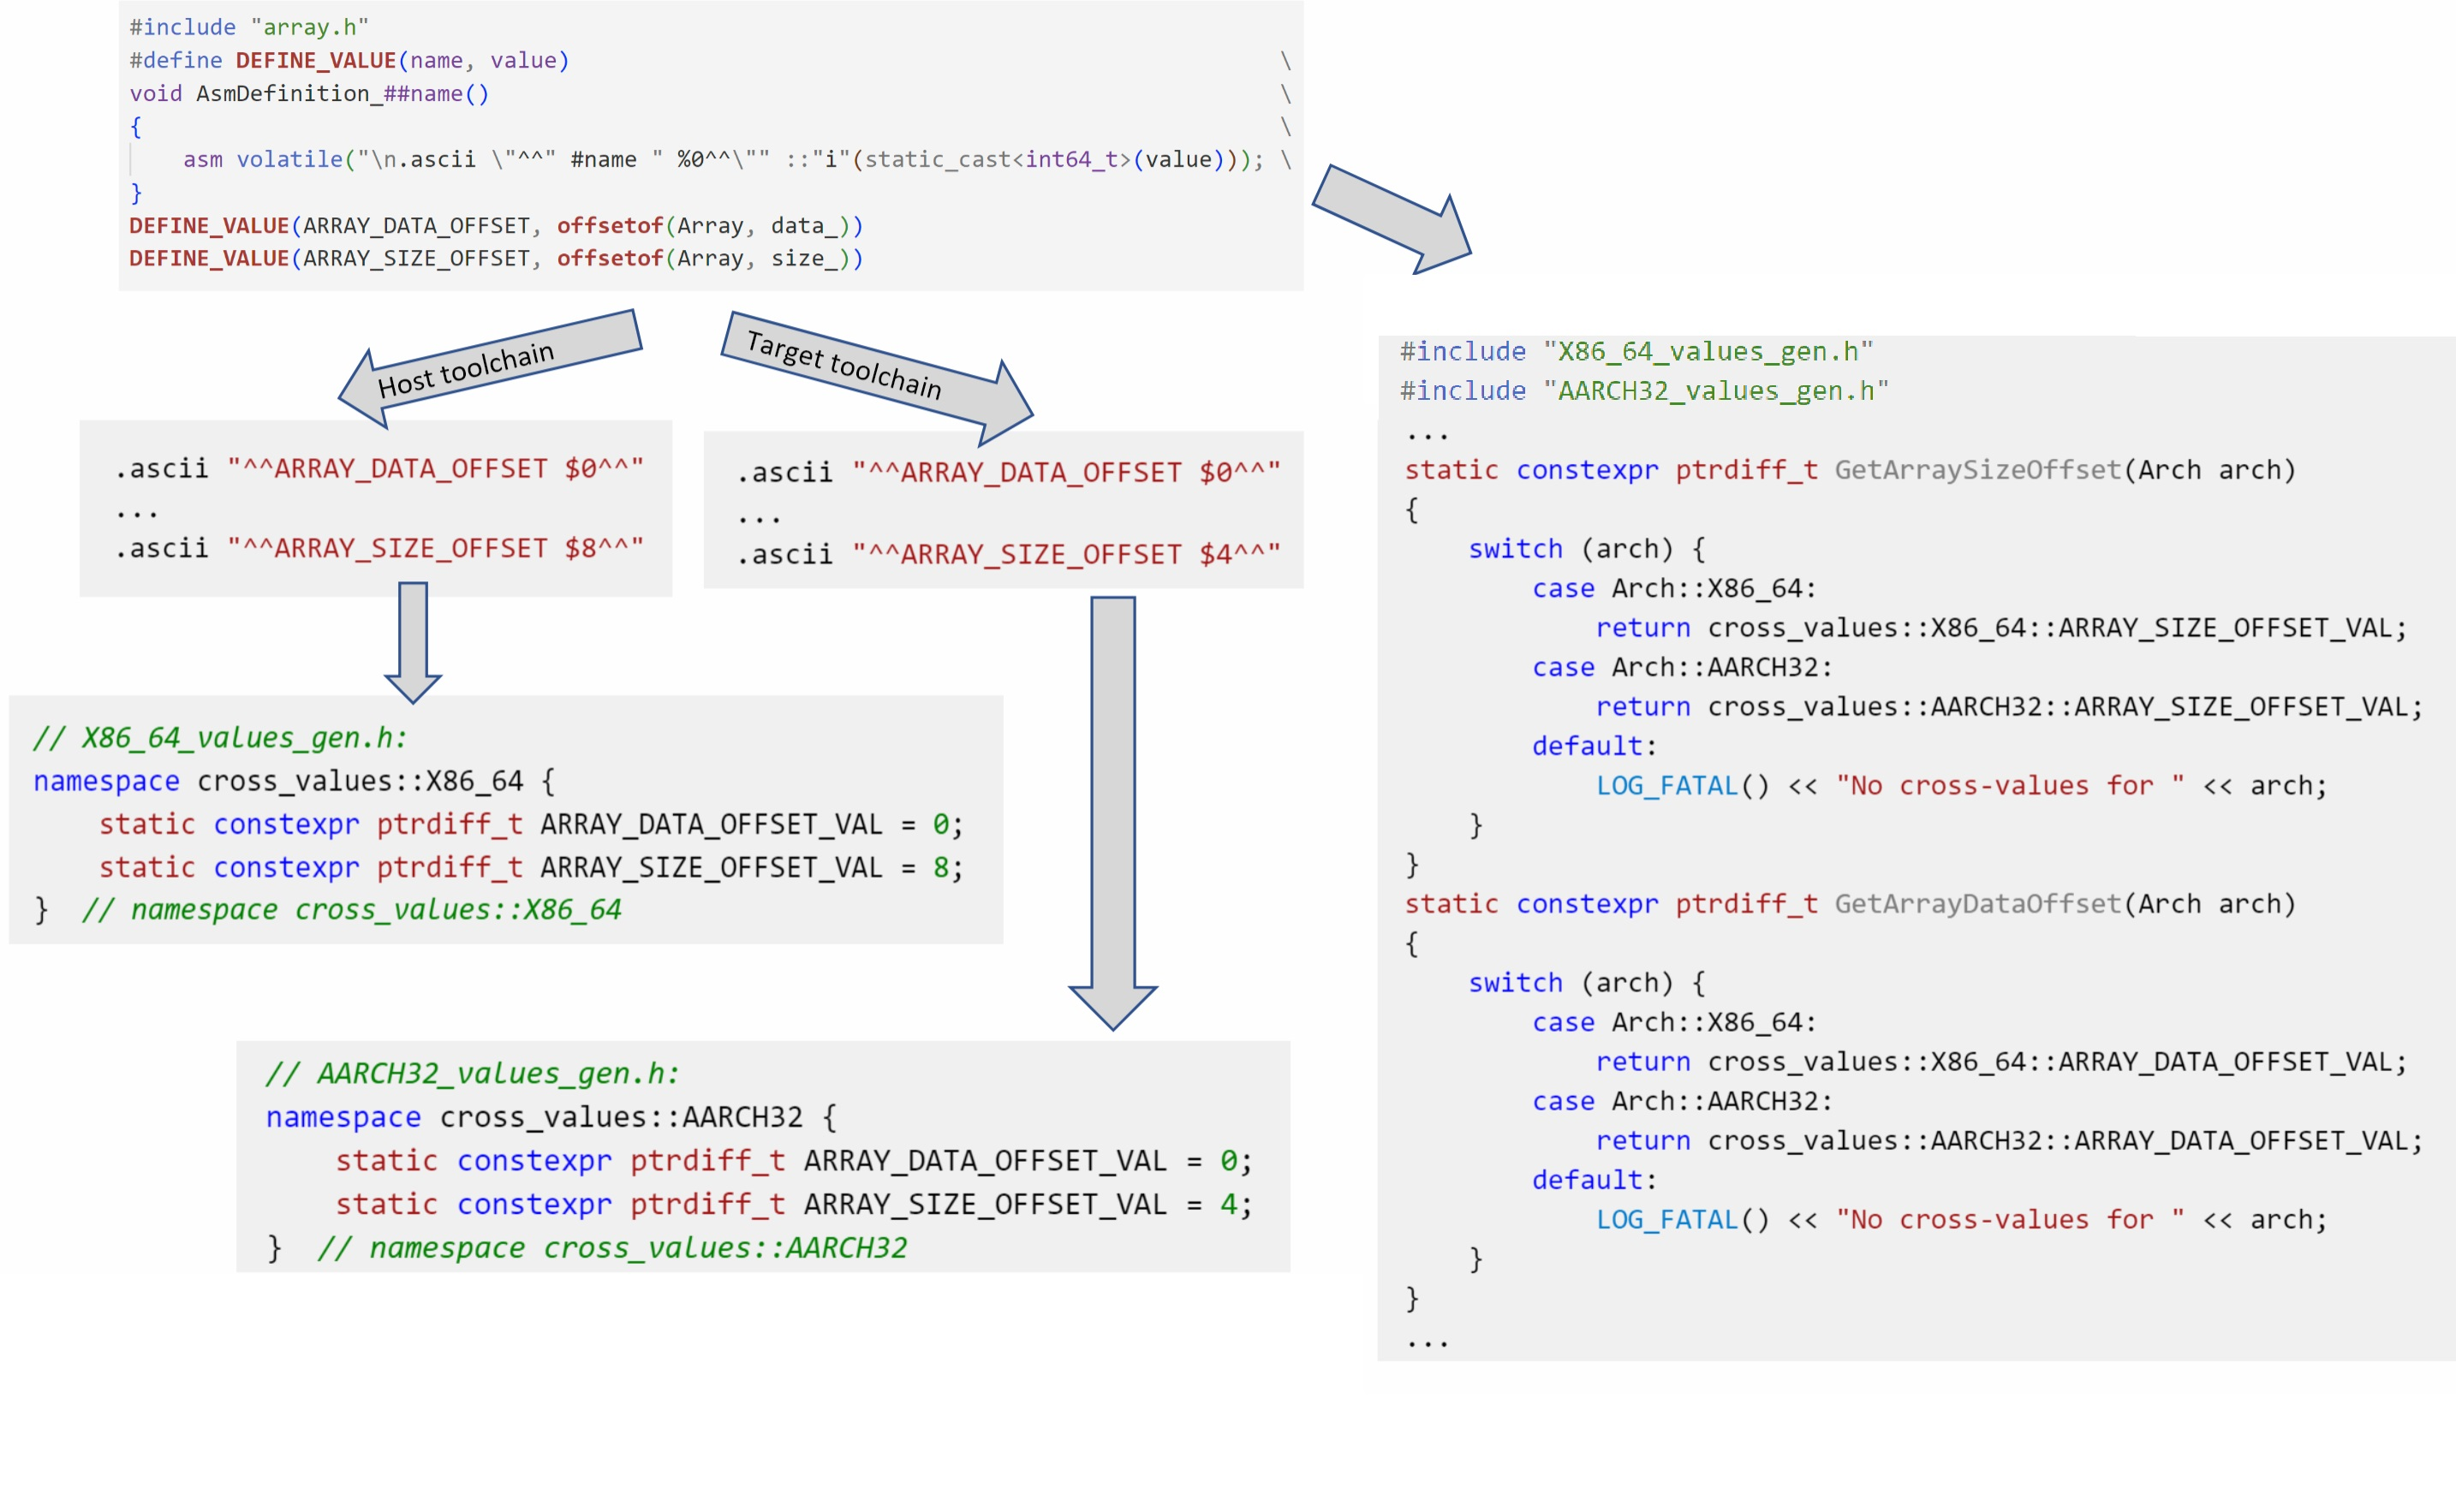
\includegraphics[scale=0.4]{asm_defines_getters.jpg}
    \caption{Схема генерации геттер-функций.}
    \label{fig:asm_defines_getters}
\end{figure}

Затем, конфигурация хост-сборки завершается и можно приступать к непосредственной сборке AOT-компилятора с помощью вызова утилиты Make \cite{make} или Ninja \cite{ninja}. Собранный таким образом компилятор располагает необходимыми значениями платформо-зависимых констант и способен генерировать корректный код для запуска в среде виртуальной машине, собранной тем же таргет-тулчейном, что и соответствующая вспомогательная директория.

\section{Детали и особенности реализации}
Основным принципом, соблюдаемым при разработке этого модуля являлось стремление к минимизации работы, связанной с его обслуживанием в будущем. В первую очередь это выражается в высоком уровне автоматизации процесса, описанного в предыдущей секции.

\par
Конфигурация вспомогательных директорий сборки происходит с использованием встроенного в \textit{CMake} модуля \textit{ExternalProject} \cite{cmake-ext-proj}.
Данный модуль позволяет встроить процессы скачивания, конфигурации, сборки и т.д. какого-то стороннего проекта в процесс сборки основного проекта, и предоставляя контроль за ними в терминах зависимостей и целей сборки.
Используя в качестве директории исходного кода стороннего проекта директорию, являющуюся деревом исходного кода для основной сборки виртуальной машины, а также указав соответствующий таргет-тулчейн образуются необходимые зависимости сборки для \textit{libasm\_defines.S} файлов (см. рис. \ref{fig:build_dir}), автоматически поддерживающие их консистентное состояние при модификациях в исходном коде.
В свою очередь, эти файлы являются входными для скриптов (см. ниже), осуществляющих генерацию файлов с определением констант в процессе сборки, а создание такой зависимости также влечёт консистентное состояние для них, в том числе. Тот факт, что они являются файлами-заголовками, позволяет построить необходимые зависимости к конечным целям сборки, включая AOT-компилятор. За счёт этого достигается корректность не только чистой сборки, но и инкрементальной, делая разработку виртуальной машины более удобной.

\par
Автоматизация обеспечивается не только с помощью \textit{CMake}, но и с помощью шаблонной генерации \textit{ERB} (сокращённо от \textit{Embedded Ruby}) \cite{erb}. Этот инструмент позволяет генерировать текстовые файлы любого формата, включая C++-код. Такой подход находит эффективное применение в обобщении однообразного кода, путём вынесения нетривиальной информации в один документ (например, \textit{JSON-} или \textit{YAML-}формата), а затем генерируя исходный код на основе его содержания по шаблону специального формата (\textit{.erb}-шаблон). К наиболее ярким его достоинствам относится явное выделение однообразия в коде (что упрощает его понимание и позволяет избежать многих ошибок, например из-за копирования кода), дешёвая с точки зрения разработки масштабируемость, возможность быстрого изменения функционала. В качестве основного документа, на основе которого производится весь описанный ранее процесс генерации, используется сама единица трансляции, изображённая на рисунке \ref{fig:asm_defines}, а также список \textit{cmake-toolchain} файлов, в том числе определяющий количество поддерживаемых AOT-компилятором платформ и сами платформы.

\par
Созданный C++-интерфейс представляет собой обычные C++-функции, имена которых основаны на именах соответствующих платформо-зависимых констант, принимающие в качестве аргумента переменную перечисляемого типа, отражающую выбранную платформу, и возвращающие значение константы на платформе согласно аргументу. Кроме того, сами константы доступны для использования непосредственно, так как находятся в отдельных пространствах имён. Это позволяет использовать данный модуль в как в платформо-определённых участках кода, так и обобщённых от платформы участках кода.

\section{Валидация}
На основе сгенерированных файлов с определениями констант вычисляется контрольная сумма.
В случае поддержки AOT-компилятором нескольких целевых платформ, контрольная сумма вычисляется для каждой из них, и соответствующее результату компиляции значение записывается в каждый выходной файл.
Аналогично, контрольная сумма записывается в образ самой виртуальной машины.
При инициализации AOT-файла происходит сравнение контрольной суммы, записанной в виртуальную машину и в AOT-файл. Это позволяет отследить ситуации расхождения констант и предотвратить ряд трудно обнаруживаемых ошибок.  

\newpage %% Исследование и построение решения задачи
    \chapter{Недостатки реализации}
\label{sec:Chapter4} \index{Chapter4}

После имплементации и интеграции описанного решения в основную ветвь проекта, проявились некоторые его тонкости, которые вполне можно отнести к недостаткам. В этой главе дан обзор этим моментам и предложены пути их сглаживания.

\section{Рассинхронизация флагов конфигурации}
Одна из существенных проблем, потенциально влекущая неконсистентность платформо-зависимых констант между кросс-компилятором и самой виртуальной машиной исходит из рассинхронизации флагов \textit{CMake}-конфигурации.
Для корректной конфигурации вспомогательных сборок важно передать все флаги, переопределённые во время инициирующего вызова \textit{cmake} из командной строки.
Если упустить какой-нибудь из них, то при конфигурации вспомогательной сборки он примет значение по-умолчанию, при этом такое различие в конфигурациях может повлиять, например, на наличие поля в какой-то структуре, смещения в которой отслеживаются рассматриваемым модулем, что повлечёт расхождение констант.
На момент написания работы, такая ошибка выявляется хотя и гарантировано, но достаточно поздно - в момент запуска приложения на устройстве.
Желательно более раннее детектирование, а в лучшем случае - предотвращение такой ошибки.
Поскольку \textit{cmake} не предоставляет интерфейса по определению флагов, указанных при вызове команды, решение может быть основанным на анализе файла \textit{CMakeCache.txt}, предназначение которого описывается в документации \textit{CMake}, содержащего действительные значения флагов. 

\section{Издержки по времени сборки}
При недостаточно аккуратно указанных зависимостях сборки проекта, возможна ситуация, при которой генерируемые файлы пересоздавались, но их содержание было бы тем же самым. Так как утилиты осуществляющие сборку (Make, Ninja) определяют модификацию файлов в терминах временных меток, а не их содержимого, это существенно замедляет инкрементальную сборку из-за лишней работы связанной с перекомпиляций, производящей в точности тот же самый результат.
Грубым решением этой проблемы будет использование утилиты на подобии \textit{ccache}.
Более правильным будет анализ зависимостей сборки и устранение ложных зависимостей.
Отсылаясь к опыту реализации и поддержки этого модуля, оказалось так, что эта проблема исходила из другой части проекта и проявлялась ранее, хотя и реже. Таким образом, анализ и исправление зависимостей привела к более предсказуемой инкрементальной сборке, устранив <<случайные>> перекомпиляции, занимающие время сравнимое с чистой сборкой проекта (т.е. около 10-20 минут).

\par
На данном этапе разработки, на конфигурацию одной вспомогательной сборки приходится около 10 секунд.
При сборке проекта с поддержкой нескольких платформ последовательная настройка может вносить некоторый дискомфорт.
Эту проблему можно решить с помощью параллелизации ценой потери информативности логов процесса конфигурации вспомогательных сборок, возможно даже совместно с их переносом из стадии конфигурации в стадию сборки основного проекта.
Это приводит к снижению наглядности процесса автогенерации и несколько усложняет трассировку проблем при ошибках конфигурации (например, связанных с инфраструктурой) для разработчика, не знакомого с этим модулем.
В этих условиях, предпочтение было сделано в пользу наглядности процесса.


\newpage %% Описание практической части
    \chapter{Заключение}
\label{sec:Chapter5} \index{Chapter5}
В процессе работы был разработан и интегрирован модуль автогенерации платформо-зависимых констант, отличающегося высокой степенью автоматизированности и масштабируемости, а также обладающего легковесным и интуитивно понятным С++-интерфейсом.
Его применение позволяет эффективно разрешить одну из проблем кросс-компиляции, то есть генерации нативного кода для гостевой платформы, в контексте AOT-компилятора виртуальной машины.
Также произведено сравнение этого решения с альтернативным, использующимся для кросс-компиляции ранее.
Выделенные достоинства и недостатки обоих подходов являются существенными доводами в пользу предлагаемого подхода.
Результатом является ожидаемое устранение критических недостатков предшествующего подхода, связанных как с вопросом корректности генерируемого кросс-компилятором кода, так и долгосрочной поддержкой проекта и внесением в него изменений.
Важно отметить, что разрешение этих проблем в первую очередь достигается именно благодаря автоматизации всего процесса.
Также выделены выявленные недостатки созданного модуля, предложены пути их устранения.  
\par
Данная работа также была представлена в рамках 65-ой Всероссийской научной конференции МФТИ.
\newpage %% Заключение

    %% Don't change the following lines
    \bibliography{references}
    \addcontentsline{toc}{chapter}{Литература}

    %% в зависимости от надобности подключаем раздел "Приложениие"
    \newpage
    \section*{Приложение}

\addcontentsline{toc}{chapter}{Приложение}
\label{sec:Apendix} \index{Apendix}
В приложении приводится основной Ruby-скрипт и использующиеся в нём ERB-шаблоны, на основе которых производится генерация C++-сущностей, описанных ранее в работе.


\lstloadlanguages{Ruby}
\definecolor{mygreen}{rgb}{0,0.6,0}
\definecolor{mygray}{rgb}{0.5,0.5,0.5}
\definecolor{mymauve}{rgb}{0.58,0,0.82}

\lstset{%
basicstyle=\ttfamily\color{black},
commentstyle = \ttfamily\color{red},
keywordstyle=\ttfamily\color{blue},
stringstyle=\color{orange}}

\lstset{ 
  backgroundcolor=\color{white},   % choose the background color; you must add \usepackage{color} or \usepackage{xcolor}; should come as last argument
  basicstyle=\footnotesize,        % the size of the fonts that are used for the code
  breakatwhitespace=false,         % sets if automatic breaks should only happen at whitespace
  breaklines=true,                 % sets automatic line breaking
  captionpos=b,                    % sets the caption-position to bottom
  commentstyle=\color{mygreen},    % comment style
  deletekeywords={...},            % if you want to delete keywords from the given language
  escapeinside={\%*}{*)},          % if you want to add LaTeX within your code
  extendedchars=true,              % lets you use non-ASCII characters; for 8-bits encodings only, does not work with UTF-8
  firstnumber=1,                % start line enumeration with line 1000
  frame=single,	                   % adds a frame around the code
  keepspaces=true,                 % keeps spaces in text, useful for keeping indentation of code (possibly needs columns=flexible)
  keywordstyle=\color{blue},       % keyword style
  language=Ruby,                 % the language of the code
  morekeywords={*,...},            % if you want to add more keywords to the set
  numbers=left,                    % where to put the line-numbers; possible values are (none, left, right)
  numbersep=5pt,                   % how far the line-numbers are from the code
  numberstyle=\color{mygray}, % the style that is used for the line-numbers
  rulecolor=\color{black},         % if not set, the frame-color may be changed on line-breaks within not-black text (e.g. comments (green here))
  showspaces=false,                % show spaces everywhere adding particular underscores; it overrides 'showstringspaces'
  showstringspaces=false,          % underline spaces within strings only
  showtabs=false,                  % show tabs within strings adding particular underscores
  stepnumber=1,                    % the step between two line-numbers. If it's 1, each line will be numbered
  stringstyle=\color{mymauve},     % string literal style
  tabsize=2,	                   % sets default tabsize to 2 spaces
  title=\lstname                   % show the filename of files included with \lstinputlisting; also try caption instead of title
}

\section{Основной скрипт}
\lstinputlisting[language=Ruby, frame=single]{code/main.rb}

\newpage
\section{Шаблон генерации численных значений}
\lstinputlisting{code/gen_constants.erb}

\newpage
\section{Шаблон генерации геттер-функций}
\lstinputlisting{code/gen_getters.erb}

\end{document}